% Record of the Econ forecast (2026 Sveriges Riksbank Prize in Economic Sciences) through step 4a.
% Compile from this folder with pdflatex (three passes), tables in tables/ are written by
% ../04_field_forecast/field_context_prompts.ipynb, figures are read from ../02_fields/results/.
\documentclass[11pt,a4paper]{article}
\usepackage[T1]{fontenc}
\usepackage[utf8]{inputenc}
\usepackage{lmodern}
\usepackage{microtype}
\usepackage[margin=24mm]{geometry}
\usepackage{booktabs}
\usepackage{array}
\usepackage{tabularx}
\usepackage{graphicx}
\usepackage{caption}
\usepackage{enumitem}
\usepackage{xcolor}
\usepackage{multirow}
\usepackage{amsmath}
\usepackage[hidelinks]{hyperref}
\graphicspath{{../02_fields/results/}}
\setlist{nosep}
\newcolumntype{L}{>{\raggedright\arraybackslash}X}
\captionsetup{font=small,labelfont=bf}
\newcommand{\code}[1]{\texttt{#1}}
\newcommand{\evtag}[1]{\textbf{[#1]}}

\title{Forecasting the 2026 Sveriges Riksbank Prize in Economic Sciences\\
\large Record of the \code{Nobel Prize/Econ} pipeline through step 4a (the field forecast prompts)}
\author{Dawoon Jeong (with Claude Code)}
\date{10 October 2026}

\begin{document}
\maketitle

\begin{abstract}
\noindent This document records the work done in \path{/project/jevans/Dawoon/Nobel Prize/Econ/} between 9 October
2026, 17:42 CDT, and 10 October 2026, about 11:30 CDT: the crawl of the complete prize record 1969--2025, the profiles
of the eleven members of the 2026 prize committee written by three language models and merged, the JEL coding of the
64 awarded works and the analysis of fields, sequence, gender and age, and the construction of the Preseen context
notes for a forecast of the \emph{field} of the 2026 prize under a design that applies field rotation strongly. It
states every design decision, the checks that were run, the numbers obtained, the costs, and what remains to be done
before the announcement on Monday 12 October 2026 (11:45 CEST at the earliest, 04:45 CDT); forecasts must be finished
by Sunday 11 October, 23:00 CDT. Later on 10 October it was extended with the results of the field forecast, the first
reference facts for the people stage (age at the award, with a data correction) and the design of the Econ virtual
committee that nominates candidates for the five leading fields.
\end{abstract}

\tableofcontents

\section{Purpose, plan and status}

The Econ folder is a forecast model for the economics prize separate from the persona experiments of
\code{../experiment/}, which covered Physiology or Medicine, Physics and Chemistry with virtual committees whose
members carried only the specialties of each committee and with options built around discoveries. The Econ model
starts from the members of the real 2026 committee and from the complete award record, and proceeds in four steps:
(1) profiles of the committee members, which may later become personas; (2) the fields the prize has gone to;
(3) candidates per field; (4) the Preseen forecast. Step 4a, the subject of the last part of this record, builds the
prompts for a Preseen question on the field; the people stage follows.

\begin{table}[h]
\small
\begin{tabularx}{\textwidth}{@{}llL@{}}
\toprule
Step & Folder & Status on 10 October 2026 \\
\midrule
Prize record 1969--2025 & \code{data/} & done 9 Oct: 57 prizes, 99 laureates, 64 works; list page and API agree on every year, name and motivation \\
1. Committee profiles & \code{01\_committee/} & done 9 Oct: 11 of 11 merged; 44 calls, \$4.66 \\
1b. Personas, discussion & -- & not started; the field question uses the profiles as context notes instead (step 4a) \\
2. Fields & \code{02\_fields/} & done 9 Oct: JEL codes of 64 works by 3 models (12 calls, \$1.52), consensus, analysis notebook executed \\
3. Candidates per field & -- & to do (people stage) \\
4a. Context notes for the field question & \code{04\_field\_forecast/} & done 10 Oct: notebook executed, 9 notes, question with 14 keyword-labelled fields \\
4b. Preseen run & \code{04\_field\_forecast/run\_field.sh} & done 10 Oct 12:00--12:44 CDT: control (no context) and main (9 notes, \code{assume\_true}), one rep each; main: Macro 16.8 \%, Trade 14.0, Production/IO 13.9, Public 12.8, Equilibrium 10.3 \\
5. Laureate reference facts & \code{05\_laureates/} & section 1 (age at the award) done 10 Oct; found and corrected the API's 2022 award-date error \\
6. Virtual committee, candidates & \code{06\_candidates/} & built 10 Oct: 11 real-member personas $\times$ 3 models, one call per cell over the five leading fields; Gemini cells running, Anthropic and OpenAI cells wait for valid keys \\
\bottomrule
\end{tabularx}
\caption{Status of the Econ pipeline. The folder is not yet tracked in the Nobel Prize git repository.}
\end{table}

\paragraph{Timeline.} Folder created 9 October 2026, 17:42 CDT. Crawl, step 1 and step 2 were built and run between
17:47 and 19:03 CDT the same day; the paid API calls ran 23:44--23:55 UTC (18:44--18:55 CDT). The step-4a notebook was
written and executed on 10 October between about 11:00 and 11:30 CDT after the design document of 9 October was
received.

\section{Shared infrastructure}

\begin{sloppypar}
\code{config.yaml} holds the dates (information cutoff \code{today: 2026-10-09}, announcement, runs-finished-by),
the names of the environment variables that hold the API keys (\code{COMMITTEE\_ANTHROPIC\_API\_KEY},
\code{OPENAI\_API\_KEY}, \code{GEMINI\_API\_KEY}, \code{PRESEEN\_API\_KEY}; the keys themselves are never stored or
printed), the three models of the 1 October virtual committees, unchanged (\code{claude-opus-5-5},
\code{gpt-5.5-2026-04-23}, \code{gemini-3.1-pro-preview}), the provider letters A, O, G used in the merged profiles,
and the prices used for cost estimates. \code{llm\_providers.py} makes JSON-mode calls to the three providers without
tools or web search. Everything runs with the Curvature interpreter called by path
(\path{/project/jevans/Dawoon/env/Curvature/bin/python}, with \code{LD\_LIBRARY\_PATH} set to its \code{lib}).
\end{sloppypar}

\section{The prize record 1969--2025 (\code{data/})}

\code{crawl\_econ\_prizes.py} fetches three sources one second apart: the nobelprize.org list page in its
\emph{All Years} view (the default view shows only 2020--2025), and the Nobel Prize API 2.1 endpoints
\code{nobelPrizes} and \code{laureates} for category \code{eco}. The page gives each year's motivation groups (a year
with two motivations was divided between two works) and the overall motivation where one exists (2025); the API adds
each laureate's share, affiliation at the prize, gender, birth and death dates. Every page laureate is matched to an
API record and the two motivation texts are compared.

\paragraph{Results of the crawl of 9 October 2026.} 57 prizes, 99 laureates (as the page states), 7 prizes divided
between two works, 3 women laureates; every motivation identical in page and API. Outputs: \code{econ\_prizes.md}
(every prize by decade with laureates, shares, motivations, affiliations), \code{econ\_prizes\_by\_year.csv},
\code{econ\_prizes\_laureates.csv} (28 columns per laureate), \code{crawl\_report.json}; the raw page and API files in
\code{raw/} with the date. Licence: API data CC0; the list page is \copyright~Nobel Prize Outreach, so the raw HTML
stays local (\code{.gitignore}). One gap: the API record of Oliver E.~Williamson has no death date (he died on
21 May 2020); the analysis notebook adds it and the crawled files stay as fetched.

\section{Step 1: profiles of the 2026 committee (\code{01\_committee/})}

\subsection{Roster}

The eleven members of the Committee for the Prize in Economic Sciences in Memory of Alfred Nobel 2026 were taken from
the nobelprize.org committee page (fetched 9 October, saved in \code{source/}); the page gives no affiliations, which
were checked against each person's university profile the same day (\code{roster.yaml}, with the link).

\begin{table}[h]
\small
\begin{tabularx}{\textwidth}{@{}llL@{}}
\toprule
Member & Role & Affiliation \\
\midrule
John Hassler & chair & IIES, Stockholm University \\
Tommy Andersson & member & Department of Economics, Lund University \\
Anna Dreber Almenberg & member & Department of Economics, Stockholm School of Economics \\
Peter Fredriksson & member & Department of Economics, Uppsala University \\
Per Strömberg & member & Stockholm School of Economics (Swedish House of Finance) \\
Timo Boppart & co-opted member & IIES, Stockholm University \\
Kerstin Enflo & co-opted member & Department of Economic History, Lund University \\
Richard Friberg & co-opted member & Department of Economics, Stockholm School of Economics \\
Randi Hjalmarsson & co-opted member & Department of Economics, University of Gothenburg \\
Jan Teorell & co-opted member & Department of Political Science, Stockholm University \\
Per Krusell & secretary & IIES, Stockholm University \\
\bottomrule
\end{tabularx}
\caption{The 2026 committee (\code{roster.yaml}).}
\end{table}

\subsection{Design and checks}

Each of the three models describes every member \emph{from its own knowledge, without web search}
(\code{prompts/ask\_system.md}, \code{ask\_user.md}; JSON schema; one call per member and model), returning an
identity check (recognized, confidence), fields with JEL codes, recent interests (period, basis), up to eight
representative works (title, year, venue, co-authors, contribution, confidence), a persona (summary, research lens,
methods and evidence, what they value in contributions, questions they would raise in deliberation, committee
experience) and knowledge limits. Claude (\code{claude-opus-5-5}, effort high) then merges the three answers into one
profile (\code{merge\_system.md}, \code{merge\_user.md}), keeping for every field, interest and work the letters of
the models that state it and the conflicts, and writing an integrated persona with a note where the models differ.
Rules in the prompts: professional information only; accuracy over completeness (a model that does not recognize
the person says so instead of guessing from the name); a work is listed only when the model is confident the title
exists; the persona is grounded in the record and does not predict whom the member will support; the merge may use
only what the three answers say.

Checks in code: every answer and merge validates against its schema (one retry on invalid JSON); support letters in
the merge must belong to answers that exist; every merged work is matched by normalized title (similarity
$\geq 0.85$) against each model's own list, the rendered badge is this checked support, a work no model listed is
marked, and a difference from the merge's own claim is shown. Every call is logged (stage, member, model, seconds,
tokens, USD).

\subsection{Results}

All eleven members were recognized by all three models with high confidence; no namesake problems were found. The
merged profiles are in \code{profiles/<slug>.md|json}, all on one page in \code{profiles/ALL.md}, one row per member
in \code{profiles/index.csv}. 44 calls (33 answers, 11 merges), \$4.66, 23:44--23:55 UTC on 9 October.

\begin{table}[h]
\small
\begin{tabular}{@{}lrrrrr@{}}
\toprule
Member & Fields & Interests & Works & Listed by all three & Listed by one model \\
\midrule
John Hassler & 6 & 6 & 9 & 2 & 3 \\
Tommy Andersson & 7 & 6 & 11 & 0 & 8 \\
Anna Dreber Almenberg & 7 & 6 & 10 & 3 & 6 \\
Peter Fredriksson & 5 & 6 & 9 & 2 & 3 \\
Per Strömberg & 6 & 8 & 10 & 3 & 3 \\
Timo Boppart & 7 & 6 & 5 & 1 & 2 \\
Kerstin Enflo & 6 & 7 & 6 & 2 & 3 \\
Richard Friberg & 5 & 5 & 11 & 1 & 7 \\
Randi Hjalmarsson & 6 & 7 & 14 & 0 & 8 \\
Jan Teorell & 6 & 6 & 11 & 2 & 5 \\
Per Krusell & 8 & 5 & 13 & 3 & 10 \\
\bottomrule
\end{tabular}
\caption{Merged profiles (\code{profiles/index.csv}): merged fields, recent interests and representative works per member, and how many works all three models or only one model listed.}
\end{table}

Known limits: what a model knows stops at its training data (roughly 2024), so recent roles and papers can be
missing or outdated; a single-model work needs checking. An earlier version of this step with web search (research,
extract, aggregate) was built and tested offline but never run, and was set aside in \code{Old/websearch\_2026-10-09/}
after the user chose the own-knowledge version.

\section{Step 2: the fields of the prize (\code{02\_fields/})}

\subsection{Design}

A \emph{work} is one motivation group of a prize year: the 57 prizes, 7 of them divided, give 64 works. Each of the
three models gives every work JEL codes from its own knowledge (\code{classify\_jel.py}; 4 batches of 16 consecutive
works, the works of a divided prize always in the same batch; the full JEL list from \code{data/classificationTree.xml}
in the prompt: 20 letters, 139 level-2 and 856 level-3 codes). Per work the model returns a \emph{primary} level-3
code (the core of the recognized contribution), up to three \emph{secondary} codes, the kind of contribution (theory,
theory and empirical, empirical, methods), whether it knows the prize beyond the motivation, and a one-sentence
rationale. Rules: code the contribution the prize recognized, not the laureates' careers; level-3 codes from the list
only; a tool that others apply (econometric, experimental, mathematical) goes under C with its first field as a
secondary code. Checks in code: the JSON schema; every work id of the batch exactly once; every code a level-3 code of
the tree, at most three secondary codes, distinct and not the primary; an invalid answer is asked once more with the
problems listed. All 12 answers were valid at the first attempt (9 October, \$1.52).

\textbf{Consensus} (\code{prize\_history.ipynb}, section 3), level by level (letter, then level 2 within it, then
level 3 within that): the code that at least two of the three primary codes share; otherwise the highest score (2 per
primary, 1 per model that lists it as secondary); a remaining tie goes to the first model in the order A, O, G.

\subsection{Results}

The three models agree on the letter for 58 of the 64 works (91\%; pairwise kappa 0.90--0.96), on the level-2 field
for 51 (80\%) and on the level-3 code for 61\%; every work has a two-model majority at the letter and level-2 levels.
Six works divide the models at the letter level: 1984 Stone (E/C), 1997 Merton--Scholes (G/C), 2009 Ostrom (D/Q),
2010 Diamond--Mortensen--Pissarides (J/D), 2019 Banerjee--Duflo--Kremer (O/C), 2025 Mokyr (N/O).

\begin{table}[h]
\small
\begin{tabularx}{\textwidth}{@{}lLrrL@{}}
\toprule
Letter & Field & Works & Prizes (share-weighted) & Years \\
\midrule
D & Microeconomics & 18 & 16.5 & 1972 \ldots\ 2020 \\
C & Mathematical and Quantitative Methods & 16 & 13 & 1969 \ldots\ 2021 \\
E & Macroeconomics and Monetary Economics & 8 & 8 & 1974 \ldots\ 2006 \\
O & Development, Innovation, Technological Change, Growth & 7 & 6 & 1971, 1979, 1987, 2018, 2019, 2024, 2025 \\
G & Financial Economics & 4 & 4 & 1990, 1997, 2013, 2022 \\
F & International Economics & 3 & 3 & 1977, 1999, 2008 \\
J & Labor and Demographic Economics & 3 & 2.5 & 2010, 2021, 2023 \\
L & Industrial Organization & 2 & 2 & 1982, 2014 \\
N & Economic History & 2 & 1.5 & 1993, 2025 \\
Q & Agricultural, Natural Resource and Environmental & 1 & 0.5 & 2018 \\
\bottomrule
\end{tabularx}
\caption{Consensus JEL letter of the 64 works. Never the main field: A, B, H, I, K, M, P, R, Y, Z (H, I, K and P appear among the secondary codes). 35 level-2 fields have won; the most frequent are O4 growth (5 works), D8 information (4) and C2 single-equation econometrics (4).}
\end{table}

\begin{figure}[h]
\centering
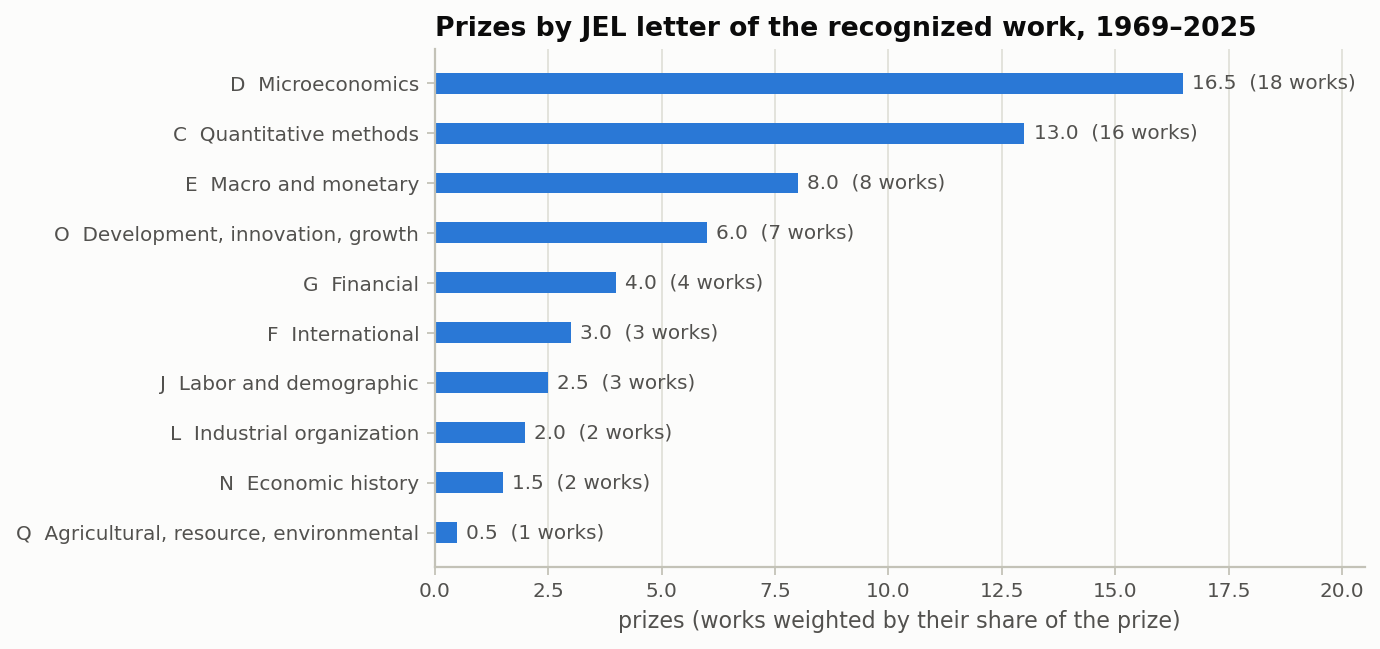
\includegraphics[width=0.49\textwidth]{fields_jel_letter.png}\hfill
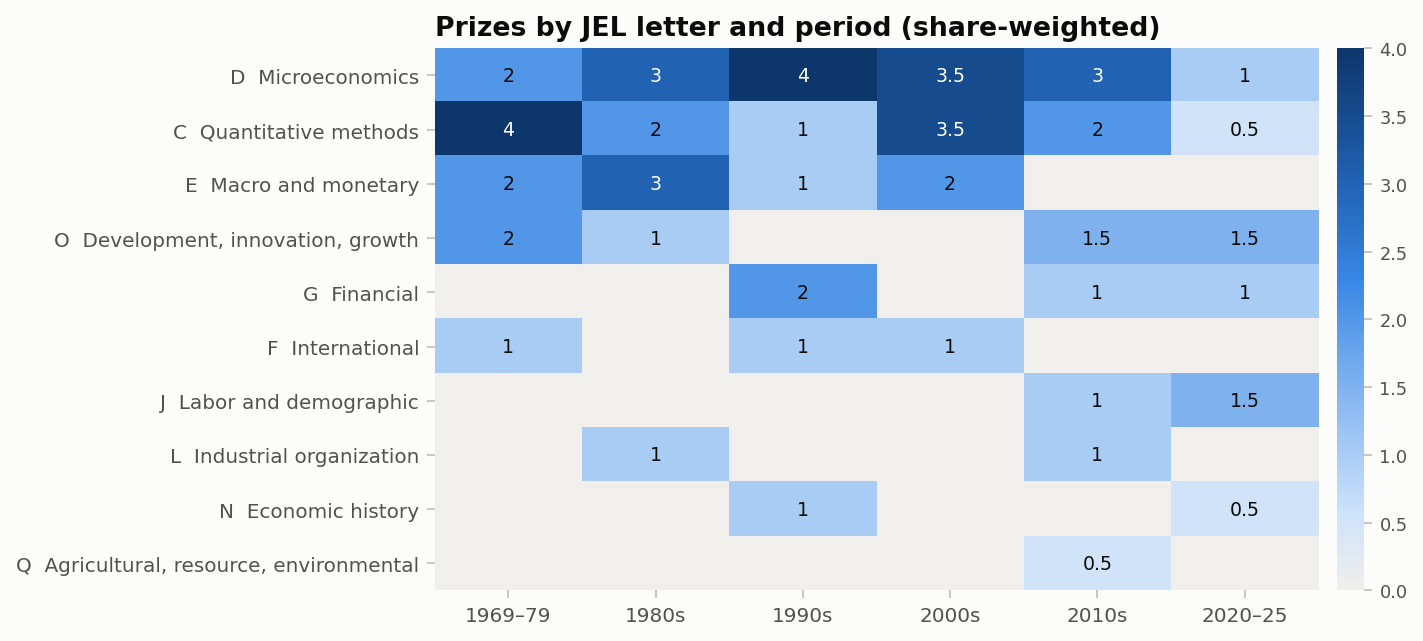
\includegraphics[width=0.49\textwidth]{fields_by_period.png}
\caption{Fields of the prize works by JEL letter (left) and by period (right); \code{02\_fields/results/}.}
\end{figure}

\paragraph{Shifts.} E was the main field eight times between 1974 and 2006 and not since (20 years against a median
gap of 3), although macroeconomics is a secondary code of 2011 (Sargent, Sims) and 2022 (Bernanke, Diamond, Dybvig)
for all three models. The last ten prizes: 2016 D, 2017 D, 2018 O+Q, 2019 O, 2020 D, 2021 C+J, 2022 G, 2023 J,
2024 O, 2025 N+O. Growth and development, labour and empirical work have gained; general equilibrium (D5, last 1988)
and mathematical modelling (C5, C6, last 1980) have not returned.

\paragraph{Sequence.} No sign that the committee avoids, or favours, the field of the year before: 10 years share a
letter with the previous year against 10.2 expected in a random order of the 57 yearly sets ($P = 0.56$; the same
for two- and three-year windows; 20,000 permutations). At level 2 a field followed itself only once (O4,
2024 $\rightarrow$ 2025; 1.5 expected). Theory and other work do not alternate more than chance (runs test
$p = 0.11$), but empirical work rose to 3 of 8 works in 2020--25.

\begin{figure}[h]
\centering
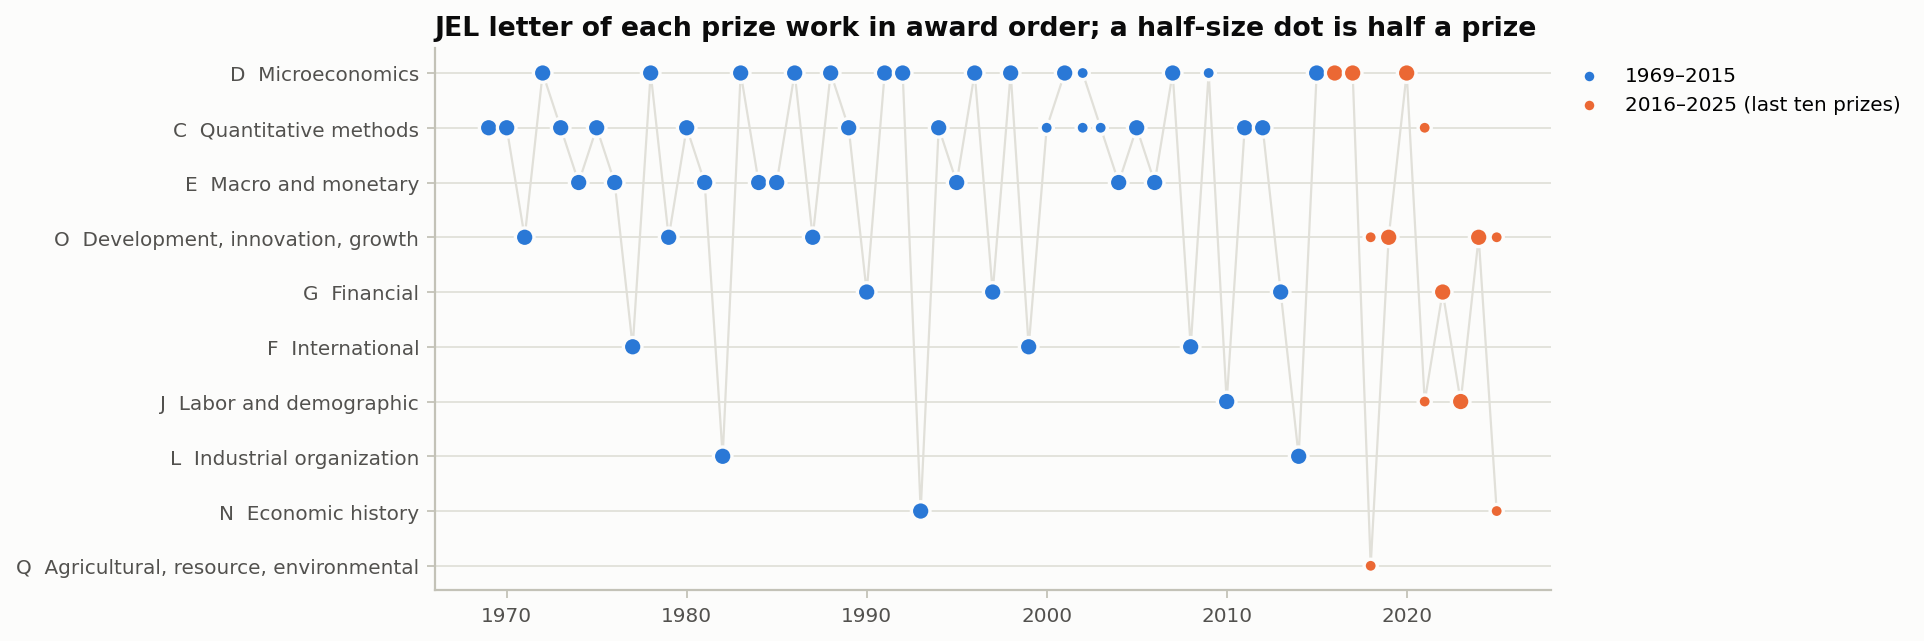
\includegraphics[width=0.56\textwidth]{field_sequence.png}\hfill
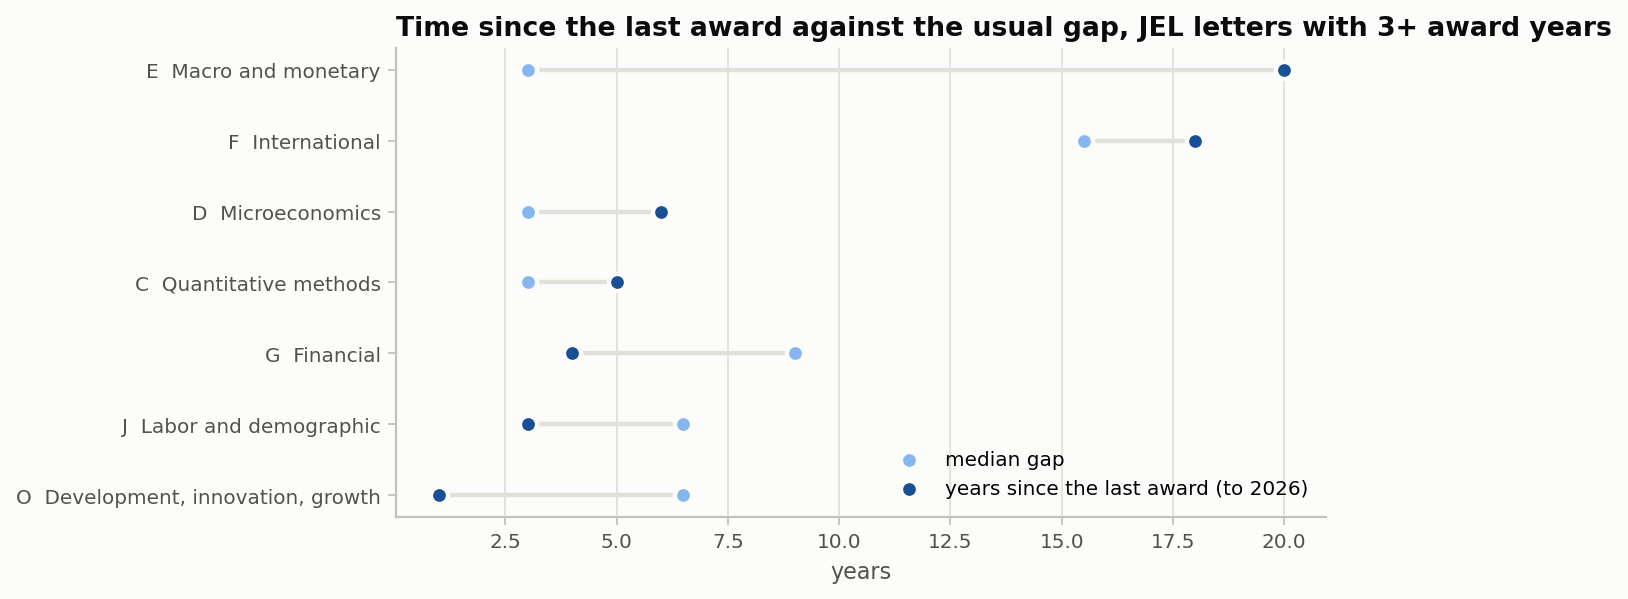
\includegraphics[width=0.43\textwidth]{field_gaps.png}
\caption{Left: the JEL letter of every prize work in award order (a half-size dot is half a prize). Right: time since the last award against the usual gap for letters with three or more award years.}
\end{figure}

\paragraph{Laureates, gender, age.} The prize is shared more and more: 1.55 laureates per prize in 1969--79, 2.0 in
the 2000s and 2010s, 2.5 in 2020--25 (one solo prize since 2020, Goldin 2023; the split 1/2 + 1/4 + 1/4 only in 2021
and 2025). 82\% of laureates had a US affiliation at the prize (at least 90\% in every period since 2000); Chicago
(15), MIT (10) and Harvard (8) lead. 3 women among 99 laureates: Ostrom (2009), Duflo (2019), Goldin (2023); since
the first, 3 of 37 (8\%). Median age at the award 67 (middle 80\%: 56--77), no trend over time ($+0.1$ years per
decade, $p = 0.81$); development and growth laureates are the youngest (median 63) and economic history and labour the
oldest (72, 70), but the field differences are not significant (Kruskal--Wallis $p = 0.60$); laureates of three-way
prizes are younger (median 64) than solo laureates (66.5) and those of two-way prizes (68). 48 of the 99 are alive
(median age 79.4; 24 are 80 or older); the others died at a median 85.9, 18.2 years after their prize.

\paragraph{Data correction (10 October).} The Nobel Prize API dates the 2022 prize (Bernanke, Diamond, Dybvig)
2011-10-10, so the crawl's integer \code{age\_at\_award} was eleven years too low for these three laureates (57, 57,
56 instead of 68, 68, 67). The error was found when the step-5 notebook recomputed ages from the dates and checked them
against the API values. The step-2 notebook now recomputes the age from the prize year where the API award date lies
outside it (the crawled file stays as fetched, as for Williamson's death date); the age figures above are the corrected
ones (the first version of this record and the step-2 summary said median 66 and ``finance youngest, median 57'',
both artefacts of the error). The context note \code{00\_5} uploaded to Preseen at 12:00 carries the API ages of the
2022 laureates; the ages are incidental to the field question. The uploaded texts are preserved in
\code{04\_field\_forecast/uploaded\_2026-10-10/} and the live notes are corrected.

\paragraph{The committee's fields against the prize fields (section 9).} A member covers a letter when one of their
merged fields carries a code in it. Members covering / prizes 1969--2025: D 10 / 16.5, C 8 / 13, J 8 / 2.5, O 6 / 6,
I 6 / 0, H 6 / 0, E 5 / 8, G 3 / 4, L 3 / 2, N 3 / 1.5, M 3 / 0, Q 2 / 0.5, A 2 / 0, K 2 / 0, R 2 / 0, F 1 / 3,
B 1 / 0, P 1 / 0. The committee covers public economics and health, education and welfare, letters never awarded as
the main field.

Outputs: \code{jel\_by\_model.csv}, \code{results/prize\_works\_jel.csv} (one row per work with the consensus at
three levels, agreement, each model's codes), \code{results/awarded\_jel\_fields.csv|md},
\code{results/field\_gaps\_letter.csv}, \code{field\_gaps\_level2.csv}, the figures, and the executed notebook
(55 cells).

\section{Step 4a: the Preseen context notes for the field forecast (\code{04\_field\_forecast/})}

\subsection{The design document}

On 10 October the user supplied a design document (written in Korean on 9 October, information date 9 October 2026,
before the announcement): \emph{Forecasting the field of the 2026 Nobel Prize in Economics: a design that applies
field rotation strongly}. It marks every statement with an evidence tag --- \evtag{P} a result reported by Dolton and
Tol (2026), \evtag{M} an opinion raised at the project meeting of 9 October 2026 (transcript \emph{E 60th St 25}, not
in the repository), \evtag{D} a design choice, \evtag{O} official sources --- and sets nine rules:

\begin{enumerate}
\item Field rotation is the most important prior: the record alone sets a baseline ranking, then the accumulation and
  maturity of unawarded work adjust it; societal attention and committee expertise are auxiliary; no field gets an
  automatic zero or a fixed turn. \evtag{D}
\item The same classification for the record and for this year's options: a project classification if one exists,
  otherwise the paper's 14 JEL-based fields; boundary rules fixed in advance; no re-labelling to avoid a penalty.
  \evtag{P, D}
\item Strong priority to the record with operational weights: awarded in the previous 1--2 years, large penalty;
  3--5 years, penalty (more if concentrated); long wait, strong bonus; these tiers are the forecast's settings, not
  thresholds the paper estimated, and related facts are not double counted. \evtag{P, D}
\item The 2023--2025 awards (Goldin; Acemoglu, Johnson, Robinson; Mokyr, Aghion, Howitt) reflected exactly, with the
  AI/employment versus growth distinction and the institutions boundary handled consistently. \evtag{O, D}
\item Check that a long-waiting field has enough mature, unawarded work with living representatives (defining
  works, long programmes, textbooks, diffusion); the paper's candidate counts are not 2026 counts. \evtag{P, M, D}
\item Societal context (AI and jobs, trade and tariffs, war and migration, inequality, institutions and democracy)
  is auxiliary; topicality does not offset a recency penalty. \evtag{M, D}
\item Committee expertise and change over time are limited adjustments; roles are distinguished; no equal votes.
  \evtag{P, O, D}
\item The paper's numbers (coefficients, pseudo-$R^2$, transition scores, individual-level regularities) are not
  this year's probabilities; information is limited to before the cutoff. \evtag{P, D}
\item A fixed output per field: representative contributions; last award, waiting time, recent frequency; baseline
  rank; maturity of unawarded work; the effect of context and committee; final rank and probability with grounds.
  \evtag{D}
\end{enumerate}

The notebook renders the document in English and adds one tag, \evtag{S}, for numbers computed from this project's
data. The user asked for a notebook in which every cell prints the text of one Preseen context note, for the
committee-profile-based field analysis to be included, and for the evidence to come from the data already completed.

\subsection{Reconciling the classifications}

Rule 2 keeps a project classification when one exists. Step 2 coded the record in JEL, which is finer than the
paper's fields in some places (E has seven awarded level-2 fields) and coarser in others (D lumps general
equilibrium, games, information and behavioural economics). The two are reconciled by taking the paper's 14 fields
(Table B.7) as the options and mapping every work into them through its consensus JEL code:

\begin{center}
\small
\begin{tabular}{@{}ll@{}}
\toprule
Field & JEL codes (Table B.7; additions in italics) \\
\midrule
Econometrics & C0--C5, \emph{C8} \\
Equilibrium, Welfare & C6, D5, D6 \\
Games, Market Structure & C7, D4 \\
Behavioural, Experimental & C9, D9 \\
Labour & D1, D3, I, J \\
Production, Industrial Organization & D2, L, \emph{M} \\
Public, Law, Political Economy & D7, H, K, P \\
Information & D8 \\
Macro & E \\
Trade & F \\
Finance & G \\
Development, Economic History & N, O1, O2, \emph{O5} \\
Growth & O3, O4 \\
Resources, Environment & Q, R \\
\bottomrule
\end{tabular}
\end{center}

Decisions \evtag{D}: C8, M and O5, absent from Table B.7, were added so that every code has a field. One work's
consensus primary code is still outside the table: Ostrom 2009 (D02, institutions); it takes the field most often
named by the three models' secondary codes --- Public, law and political economy (H41, D71: 5 of 7 mentions; Q20:
2). The 2024 prize (O43, institutions and growth) is Growth, with its secondary codes (P16, N40, D02) showing the
overlap with Public and Development; mechanism design (D82) is Information, auction and matching design (D44, C78)
Games; household, health and education economics are Labour; urban and regional economics are Resources. The
notebook asserts that all 64 works map and that the prizes sum to 57.

\subsection{The record in the 14 fields}

Table~\ref{tab:h14} is the baseline from the record alone (rule 3): the fields ordered by years since the last award,
ties broken by fewer prizes in 2016--2025 and then fewer prizes overall; the tier is the design's operational weight.
It differs from the JEL-letter view of step 2 in instructive ways: Microeconomics (D, 16.5 prizes, last 2020) splits
into Equilibrium and welfare (last 1998), Games (2020), Information (2016), Behavioural (2017) and parts of Labour,
Production and Public; the letter C splits into Econometrics (last 2021) and the mathematical methods of the 1970s,
which join Equilibrium. The same field followed itself in 3 of 56 transitions (1973 Equilibrium, 1985 Macro, 2025
Growth), against 10 of 56 at the letter level.

\begin{table}[h]
\centering
\small
\resizebox{\textwidth}{!}{\begin{tabular}{@{}rlrrlrrrr@{}}
\toprule
Rank & Field (JEL) & Prizes & Last & Since & Median gap & 2021--25 & 2016--25 & Tier \\
\midrule
1 & Equilibrium, Welfare (C6, D5, D6) & 7.0 & 1998 & 28 & 3.5 & 0.0 & 0.0 & bonus \\
2 & Macro (E) & 8.0 & 2006 & 20 & 3 & 0.0 & 0.0 & bonus \\
3 & Trade (F) & 3.0 & 2008 & 18 & 15.5 & 0.0 & 0.0 & bonus \\
4 & Public, Law, Political Economy (D7, H, K, P) & 1.5 & 2009 & 17 & 23 & 0.0 & 0.0 & bonus \\
5 & Production, Industrial Organization (D2, L, M) & 4.5 & 2014 & 12 & 7 & 0.0 & 0.0 & bonus \\
6 & Information (D8) & 4.0 & 2016 & 10 & 6 & 0.0 & 1.0 & neutral \\
7 & Behavioural, Experimental (C9, D9) & 2.0 & 2017 & 9 & 15 & 0.0 & 1.0 & neutral \\
8 & Resources, Environment (Q, R) & 0.5 & 2018 & 8 & -- & 0.0 & 0.5 & neutral \\
9 & Games, Market Structure (C7, D4) & 4.0 & 2020 & 6 & 8 & 0.0 & 1.0 & neutral \\
10 & Econometrics (C0-C5, C8) & 6.5 & 2021 & 5 & 9.5 & 0.5 & 0.5 & penalty \\
11 & Finance (G) & 4.0 & 2022 & 4 & 9 & 1.0 & 1.0 & penalty \\
12 & Labour (D1, D3, I, J) & 4.5 & 2023 & 3 & 5.5 & 1.5 & 1.5 & penalty \\
13 & Development, Economic History (N, O1, O2, O5) & 3.5 & 2025 & 1 & 14 & 0.5 & 1.5 & large penalty \\
14 & Growth (O3, O4) & 4.0 & 2025 & 1 & 11 & 1.5 & 2.0 & large penalty \\
\bottomrule
\end{tabular}
}
\caption{The 64 prize works in the 14 fields (share-weighted prizes; years since the last award to 2026; median gap
between award years; prizes in 2021--25 and 2016--25; operational tier of the design). Written by the step-4a
notebook to \code{tables/fields14\_history.tex}.}
\label{tab:h14}
\end{table}

\subsection{Committee coverage of the fields}

Each member's profile fields carry JEL codes; a member covers a field when one of their profile fields has a code in
it, and the mark is filled when at least two of the three models state that profile field. The main field of a member
is the field with the largest support-weighted number of codes. For comparison, Dolton and Tol's Table A.6 assigns
one field and one JEL code to every committee member of 1969--2025, including the 2025 roster, which has the same
eleven people as 2026 (Table~\ref{tab:c14}).

\begin{table}[h]
\centering
\small
\resizebox{\textwidth}{!}{\begin{tabular}{@{}llccccccccccccccl@{}}
\toprule
Member & Role & Em & Eq & Gm & Bh & Lb & IO & Pb & In & Ma & Tr & Fi & Dv & Gr & Re & Dolton--Tol A.6 \\
\midrule
John Hassler & chair (member) &  & $\bullet$ &  &  & $\bullet$ &  & $\bullet$ &  & $\bullet$ &  &  &  & $\bullet$ & $\bullet$ & Growth (O4) \\
Tommy Andersson & member &  & $\bullet$ & $\bullet$ &  & $\bullet$ &  & $\bullet$ & $\bullet$ &  &  &  &  &  & $\bullet$ & Information (D8) \\
Anna Dreber Almenberg & member & $\bullet$ & $\circ$ & $\circ$ & $\bullet$ & $\bullet$ &  &  & $\bullet$ &  &  & $\bullet$ &  &  &  & Behavioural (D9) \\
Peter Fredriksson & member & $\bullet$ &  &  &  & $\bullet$ & $\circ$ & $\bullet$ & $\bullet$ & $\bullet$ &  &  &  &  &  & Labour (I2) \\
Per Strömberg & member &  &  & $\bullet$ &  &  & $\bullet$ & $\bullet$ & $\bullet$ &  &  & $\bullet$ & $\circ$ &  &  & Finance (G2) \\
Timo Boppart & co-opted &  & $\bullet$ &  &  & $\bullet$ & $\bullet$ &  &  & $\bullet$ &  &  & $\bullet$ & $\bullet$ &  & Trade (F2) \\
Kerstin Enflo & co-opted & $\bullet$ &  &  &  & $\circ$ &  &  &  & $\bullet$ &  &  & $\bullet$ & $\bullet$ & $\bullet$ & Development (N1) \\
Richard Friberg & co-opted &  &  &  &  & $\circ$ & $\bullet$ & $\circ$ & $\bullet$ &  & $\bullet$ & $\bullet$ &  &  &  & Labour (I2) \\
Randi Hjalmarsson & co-opted & $\bullet$ &  &  & $\bullet$ & $\bullet$ &  & $\bullet$ &  &  &  &  & $\circ$ &  &  & Labour (I2) \\
Jan Teorell & co-opted & $\bullet$ &  &  &  &  &  & $\bullet$ &  &  &  &  & $\bullet$ & $\bullet$ &  & Public (D7) \\
Per Krusell & secretary &  & $\bullet$ &  & $\circ$ & $\bullet$ &  & $\bullet$ &  & $\bullet$ &  &  &  & $\bullet$ & $\bullet$ & Growth (O4) \\
\midrule
members covering & & 5 & 5 & 3 & 3 & 9 & 4 & 8 & 5 & 5 & 1 & 3 & 5 & 5 & 4 & \\
\bottomrule
\end{tabular}
}
\caption{Coverage of the 14 fields by the 2026 committee according to the step-1 profiles ($\bullet$ stated by 2--3 models, $\circ$ by one), with Dolton and Tol's one-field assignment. Em econometrics, Eq equilibrium, Gm games, Bh behavioural, Lb labour, IO production and IO, Pb public, In information, Ma macro, Tr trade, Fi finance, Dv development and economic history, Gr growth, Re resources.}
\label{tab:c14}
\end{table}

Labour (9 members) and Public, law and political economy (8) are the most covered fields; Trade is covered by one
member (Friberg, through pricing-to-market and exchange-rate pass-through); Econometrics, Equilibrium, Information,
Macro, Development and Growth by five each. Main fields by the profiles: Hassler and Krusell Macro, Andersson Games,
Dreber Almenberg Behavioural, Fredriksson and Hjalmarsson Labour, Strömberg Finance, Boppart Growth, Enflo
Development and economic history, Friberg Production and IO, Teorell Public. The paper's assignment differs for
Boppart (Trade, F2, against growth and structural change in the profiles) and Friberg (Labour, I2, against industrial
organization and international pricing); for Hassler and Krusell it says Growth (O4) where the profiles put macro
first with growth, climate and public economics beside it. The notes use the coverage only as the limited adjustment
of rule 7.

\subsection{The notes}

\begin{table}[h]
\small
\begin{tabularx}{\textwidth}{@{}lLl@{}}
\toprule
File & Content & Tags \\
\midrule
\code{00\_1\_instruction} & goal, evidence tags, the rotation prior, the operational weights, pointers to the reference notes, the required output; written for the \code{assume\_true} treatment & P M D \\
\code{00\_2\_field\_classification} & the 14 fields and their codes, the additions, the boundary rules & P D \\
\code{00\_3\_prize\_works\_by\_field} & every prize work 1969--2025 in its field: year, laureates, share, consensus code and JEL name, fallback rule, other fields the secondary codes point to & S O \\
\code{00\_4\_prize\_history\_by\_field} & Table~\ref{tab:h14} as a markdown table; sequence facts & S \\
\code{00\_5\_recent\_prizes\_2021\_2025} & the seven works of 2021--2025 with laureates, shares, affiliations, ages, official motivations, the three models' codes, field and weight; how to read them & O S D \\
\code{00\_6\_unawarded\_maturity} & what to assess; the paper's pool sizes per field (Table B.7) and why they are not 2026 counts; what the project does not provide & P M D \\
\code{00\_7\_societal\_context} & the meeting's themes as auxiliary information & M D \\
\code{00\_8\_committee\_2026} & roster and roles, the coverage table, one line per member, how to use it & O S P D \\
\code{00\_9\_paper\_evidence\_and\_limits} & the paper's field-level results and the limits of using them & P D \\
\bottomrule
\end{tabularx}
\caption{The context notes in \code{04\_field\_forecast/context/}. Sizes 1.1k--9.7k characters, 44k in all; attached in name order, all with \code{treatment=assume\_true}.}
\end{table}

\paragraph{What was checked in the paper.} The arXiv PDF (4.3 MB) was fetched on 10 October and its text extracted
to read the figures quoted in the notes: Table B.7 (the 14 fields with candidates and laureates per field), Table 2
(field-level logit over 798 field-years: number of candidates 19.84, $p<0.001$; transition probability with and
without Lindbeck 75.76, $p<0.001$; years since the field last won 0.0576, $p<0.01$; year 0.0249, $p<0.05$; won in
the previous year 0.066 with the matrix and $-1.78$ without, both insignificant; log-likelihood $-137$ against $-198$
and pseudo-$R^2$ 37\% against 9.1\% without the matrix), Table A.6 (committee members' fields) and the text on the
sample split at 1997 (Table E.12: optimal age 71.4 then 70.8; committee proximity significant only in the second
half; citation indicators significant only in the first). The design document's ``39 years after the PhD'' was not
checked and is not quoted.

\paragraph{An external-signals note, built and dropped.} A tenth note was built in the first version of the
notebook from \code{Data/convergence\_2026.csv}, which holds, for all four prizes, people with convergent external
signals collected before the 2026 science prizes; its 58 economics rows carry 40 Nobel symposium dossier entries
(2022 inequality, 2022 social network analysis, 2026 international economics), 12 entries from 2026 web prediction
lists, 9 Kalshi prices (KXNOBELECON: Pakes 0.26, Athey 0.16, Blundell 0.08, Barro 0.07, Fehr, Mas-Colell and Dasgupta
0.06, Rabin 0.05, Zingales 0.02), 4 Clarivate 2026 citation laureates (Woodford, Athey, Varian, Winter), 8
high-predictive-value prizes (BBVA Frontiers 2024 and 2025, Nemmers 2024 and 2026, Clark Medals 2024--2026) and 2
Swedish proximity signals, each person given a field by the author from general knowledge. On 10 October the user
decided to exclude it entirely (not even with the weaker \code{consider} treatment): information about named people
is the channel the design wants to keep out of the field stage, and the field assignments were the author's. The cell
was removed from the notebook and the run script refuses to start unless \code{context/} holds exactly the nine
\code{00\_} notes.

\subsection{The question}

\code{questions/fields14.json}: multiple choice, ``Which field of economics will the 2026 Sveriges Riksbank Prize in
Economic Sciences recognize?'', 14 options of the form \code{<field> (JEL <codes>): <three or four keywords>}
(for example ``Information (JEL D8): asymmetric information, contract theory, mechanism design, decision making under
uncertainty''), mutually exclusive and comprehensive, no Other. Three points were settled in discussion with the user
on 10 October before submission. (i) Keywords were added to the labels so that the forecaster and the resolver read
the same boundaries; the fine print says the keywords are illustrative and the JEL code groups define the fields.
(ii) The resolution procedure is pre-committed: the primary code of the 2026 motivation is determined by the same
three-model JEL coding and consensus rule that coded 1969--2025 and mapped by the code groups of the labels, so no
judgment is exercised after the announcement. (iii) A prize divided between fields resolves by the overall motivation
when the announcement gives one, otherwise by the larger share, then by the contribution named first; the earlier
draft (larger share, then first named) would have resolved the 2025 prize to Development and economic history through
Mokyr's first-named half although the overall motivation, ``innovation-driven economic growth'', is Growth. A primary
code outside the 14 fields resolves by the majority of the secondary codes; if no field can be assigned the question
is annulled. The instruction note states the same event so that the forecast and the resolution refer to one thing.

\subsection{Treatments and arms}

Preseen attaches a context note with a treatment. In this project's earlier runs \code{assume\_true} behaved as a
premise to apply (a note excluding one person from the Medicine forecast was applied; the Chemistry instruction notes
moved the ranking to Spearman 0.14--0.39 against control), while \code{consider} behaved as one input among many
(person cards attached only as \code{consider} left the Medicine and Physics forecasts close to control). The nine
notes are therefore attached as \code{assume\_true}: the brief (00\_1) only bites as a premise, the classification
and the record (00\_2--00\_5) define the event, and 00\_6--00\_9 are the rest of the design; the committee note is
the weakest fact but its own text restricts it to a limited adjustment. Two arms with identical private questions were
submitted on 10 October (\code{run\_field.sh}, tag \code{nobel26-econ-fields}, one rep each): \emph{control} without
context, which gives Preseen's own view of the field, and \emph{main} with the nine notes. Possible further arms,
not submitted: all notes as \code{consider} (how much the strong-rotation premise drives the result), a second rep
of each arm (run-to-run noise).

\subsection{Execution}

The notebook \code{field\_context\_prompts.ipynb} (31 cells) was generated from a script and executed with
\code{nbconvert} on the login node (kernel \code{curvature}, about two minutes, no paid calls). The notebook asserts the input counts (64
works, 99 laureates, 11 valid profiles), the complete mapping, the prize total, and that every person of the
convergence file has an assigned field; it writes the notes, the question, \code{results/*.csv} and the two LaTeX
tables of this record. Nothing was uploaded to Preseen.

\subsection{Results of the field forecast}

Both runs completed on 10 October: control in 27 minutes (4 subforecasts, 357 sources consulted), main in 44 minutes
(4 subforecasts, 465 sources). Table~\ref{tab:res14} sets the two distributions beside the record-only baseline.

\begin{table}[h]
\centering
\small
\resizebox{\textwidth}{!}{\begin{tabular}{@{}lrlrrrr@{}}
\toprule
Field & Baseline rank & Tier & Control \% & Main \% & Main $-$ control (pp) & Main rank \\
\midrule
Macro & 2 & bonus: & 14.5 & 16.8 & +2.3 & 1 \\
Trade & 3 & bonus: & 6.8 & 14.0 & +7.2 & 2 \\
Production, Industrial Organization & 5 & bonus: & 14.6 & 13.9 & -0.7 & 3 \\
Public, Law, Political Economy & 4 & bonus: & 3.4 & 12.8 & +9.4 & 4 \\
Equilibrium, Welfare & 1 & bonus: & 3.7 & 10.3 & +6.6 & 5 \\
Information & 6 & neutral & 8.2 & 6.5 & -1.7 & 6 \\
Resources, Environment & 8 & neutral & 3.8 & 6.3 & +2.5 & 7 \\
Behavioural, Experimental & 7 & neutral & 6.3 & 5.8 & -0.5 & 8 \\
Games, Market Structure & 9 & neutral & 7.5 & 4.4 & -3.1 & 9 \\
Econometrics & 10 & penalty & 12.3 & 3.1 & -9.2 & 10 \\
Labour & 12 & penalty & 9.5 & 2.3 & -7.2 & 11 \\
Finance & 11 & penalty & 3.8 & 2.2 & -1.6 & 12 \\
Development, Economic History & 13 & large & 2.7 & 0.9 & -1.8 & 13 \\
Growth & 14 & large & 2.8 & 0.7 & -2.1 & 14 \\
\midrule
bonus tier (5 fields) &  &  & 43.0 & 67.8 &  &  \\
penalty tiers (5 fields) &  &  & 31.1 & 9.2 &  &  \\
\bottomrule
\end{tabular}
}
\caption{Preseen's probability per field, control (no context) against main (nine notes as \code{assume\_true}),
with the record-only baseline rank and tier of Table~\ref{tab:h14}. Spearman main--control 0.43, main--baseline
0.94, control--baseline 0.27; entropy main 2.36, control 2.48, uniform 2.64.}
\label{tab:res14}
\end{table}

\begin{itemize}
\item \textbf{The brief was followed.} The main write-up reports the three distributions the instruction asked for:
  a record-only distribution from its own operational formula, $(\text{wait}+5)^{0.8} \times \text{tier} /
  (1 + 0.10 \times \text{ten-year shares})$ with tiers 1.25 / 1.00 / 0.60 / 0.40, then a maturity factor $M$ per field
  (Production and IO 1.75 for structural empirical IO; Macro 1.60 for the New Keynesian programme; Trade 1.45 for
  heterogeneous-firm trade; Public 1.40; Equilibrium 0.85 and Growth 0.90 as the only discounts), then small auxiliary
  factors for societal relevance, committee expertise and dated recognition (none above 1.08). It restates that
  strong rotation is a modelling assumption and that the paper's transition matrix is not used as probabilities.
  Its final ranking correlates 0.94 with the record-only baseline; the five bonus-tier fields hold 67.8 \% (control
  43.0 \%), the 2021--2023 tier 7.6 \% (25.6 \%), the 2024--2025 fields 1.6 \% (5.5 \%).
\item \textbf{Preseen's own view (control)} leads with Production and IO 14.6 \%, Macro 14.5, Econometrics 12.3,
  Labour 9.5. It built its own contribution-first coding of the 57 prizes, which differs from the step-2 coding in
  several assignments (Ostrom to Resources, the 2010 search prize to Information, the 2024 prize to Growth with
  Development at three awards), and it put the historical component below the contribution assessment.
\item \textbf{Where the arms agree and differ.} Macro is first in both arms (16.8 against 14.5) and Production and
  IO is in the top three of both; the notes move Public (3.4 to 12.8), Trade (6.8 to 14.0) and Equilibrium (3.7 to
  10.3) up and Econometrics (12.3 to 3.1) and Labour (9.5 to 2.3) down. Both distributions stay flat: no field
  exceeds 17 \%.
\item \textbf{External signals entered anyway.} Although the external-signals note was excluded, the main run found
  the same signals by its own search (Woodford's Clarivate 2026 listing, the BBVA 2025 prize to Blanchard, Gal\'i and
  Woodford, the Academy's 2026 and 2027 Nobel symposia on international economics) and used them as the small factor
  $R$; the control run used them more.
\item \textbf{Resolution.} After the announcement on 12 October the motivation is coded with \code{classify\_jel.py}
  (three models, consensus) and mapped by note 00\_2; the log score of each arm over the 14 options is then recorded
  here. The write-ups are saved in \code{04\_field\_forecast/results/write\_up\_\{control,main\}.md}.
\end{itemize}

\section{Step 5: reference facts from the laureate record (\code{05\_laureates/})}

The people stage needs priors from the record of the 99 laureates. \code{laureate\_history.ipynb} collects them
section by section; each section ends with an English paragraph written to \code{prompt/<section>.md} for later use
as a context note. Section 1 (10 October) covers the age at the award.

\paragraph{Age at the award.} Age is computed from the birth date to the announcement (four laureates have a birth
year only). Median 67 (bootstrap 95\% 64--69), mean 67.3, standard deviation 8.3, middle 80\% 57--78; 4 laureates under
55 (Duflo 47, Arrow 51, Merton 53, Kremer 55), 6 aged 80 or more (Hurwicz 90, Shapley 89, Schelling 84, Wilson 83,
Vickrey 82, Coase 81). The distribution has one peak: a Gaussian mixture prefers one component by BIC, skewness
$+0.34$, Shapiro--Wilk $p = 0.48$; the mode of the density is 65 (bootstrap 62--69). Two readings of ``optimal age''
are distinguished: the mode of the laureate distribution (65--67) and the age at which a \emph{candidate} is most likely
to win, which Dolton and Tol estimate on their candidate pool at 70--71 [P]. Without their pool the notebook computes
the award rate among eventual laureates (of those not yet awarded at age $a$, the share awarded at $a$): it passes 5\%
at 61 and 10\% at 68 and peaks around 77 among ages with at least ten laureates still unawarded, but it rises
mechanically as the pool empties. The honest reading is a broad plateau from 60 to 77 rather than a sharp optimum.
No trend over time ($+0.13$ years per decade, $p = 0.80$; 1969--1997 median 66, 1998--2025 median 67). By field the
medians run from Information 61 and Growth 64 to Labour 70 and Games 74 (Kruskal--Wallis $p = 0.37$); three-way
prizes go to younger people (median 64) than two-way prizes (69) and solo prizes (67) ($p = 0.07$). Co-laureates of one
work differ in age by a median of 9 years; 4 of 26 shared works have a gap of 15 years or more (Hurwicz--Maskin--Myerson
34, Roth--Shapley 29, Mirrlees--Vickrey 22, Hicks--Arrow 17). Of the 51 deceased laureates the median died at 86, 18
years after the prize; 7 died within five years; of the 20 awarded at 75 or older, 13 have died, after a median of 11
years. The paragraph for the people stage (\code{prompt/01\_age\_at\_award.md}) concludes that a candidate's age
matters mostly at the extremes (under 55 and 80 or over are rare) and that co-laureates are usually of one generation.
The notebook is where the API's 2022 award-date error was found (the exact ages were checked against the API's
integer ages and three disagreed by eleven years); see the data correction in the step-2 section.

\section{Step 6: the Econ virtual committee (\code{06\_candidates/})}

\subsection{Purpose and design choice}

The people stage starts from candidate pools per field, larger for the fields with the higher forecast probability. As
for Physics, Chemistry and Medicine, a virtual committee nominates the candidates; unlike those committees, whose
personas carried only the specialties of the real members, the Econ committee's eleven personas are the real 2026
members as reconstructed in step 1. The user chose, on 10 October, the design in which one call per member and model
covers all five fields (33 cells) over the alternative of one call per member, model and field (165 cells). The
nominations of the three models are then integrated into one candidate list per field by claude-opus-5-5 (the user's
choice over the rule-based clusters and a hand-made \code{merges.yaml}), and the lists become Preseen context notes for
the people question.
\code{virtual\_committee.py} is written for the Econ pipeline and imports nothing from \code{experiment/}; the
functions of the 1 October script that apply unchanged were copied into it (listed below).

\begin{table}[h]
\small
\begin{tabularx}{\textwidth}{@{}lLL@{}}
\toprule
 & 1 October committees (Med, Phys, Chem) & Econ \\
\midrule
Personas & specialties of the real committee, anonymous & the 11 real members, from the merged step-1 profiles (summary, research lens, methods and evidence, what they value, questions they would raise, fields, recent interests) \\
Cells & persona $\times$ model, one ballot per field (66 cells) & member $\times$ model, one call over the five fields (33 cells) \\
Nominations & $\leq 5$ ranked per ballot & $\leq 5$ ranked per field, $\leq 25$ per cell \\
Nomination & discovery line, 1--3 living people with affiliation, $\leq 3$ key papers, rationale $\leq 2$ sentences & the same, plus the JEL level-3 code of the contribution and each person's year of birth \\
Models & claude-opus-5-5, gpt-5.5-2026-04-23, gemini-3.1-pro-preview; no tools, no web search, provider defaults, 32k output cap & the same \\
Validation & JSON schema, one retry, count limits as warnings & the same, plus every field present once, and a warning when a code lies outside the field's groups \\
Aggregation & model-balanced Borda 5..1, person-key clustering, reviewed \code{merges.yaml} & model-balanced Borda 5..1 per field; grouping of the nominations into candidates by claude-opus-5-5 (\code{integrate}); supporters by member and role, per-person support and flags computed locally \\
Output & top-$K$ options and ``Other'' & one Preseen context note per field (candidates with lineup, defining works, reasoning and support), and a 30-option pool allocated to the fields in proportion to the main-arm probability \\
\bottomrule
\end{tabularx}
\caption{The Econ virtual committee against the 1 October committees.}
\end{table}

\subsection{Fields, prompt and schema}

The five fields are those with the highest probability in the main (treatment) arm of the latest field run, the
second experiment with the title ``Which field of economics will the 2026 Nobel Prize in Economic Sciences recognize?''
(task \code{9b0a6220}, finished 13:51 CDT): Macro 16.9\%, Trade 15.6\%, Production and IO 14.0\%, Public, law and
political economy 13.3\%, Equilibrium and welfare 9.5\% (\code{settings.yaml}; the first experiment had the same five
in the same order, 16.8/14.0/13.9/12.8/10.3). On the user's request the committee was briefly set up for all 14 fields
in three batches (5/5/4 fields per call; the nine further definitions follow the boundary rules of note 00\_2 and the
awarded record), then restricted to the five leading fields; the other nine stay in \code{settings.yaml} with
\code{batches\_to\_ask: [1]} and enter the prompt only as the list of the 14 fields with their codes, which fixes the
boundaries. Each field carries a definition with its boundary rules (from note 00\_2) and the list of the
works already awarded in it, with the official motivations and the consensus code of step 2, from
\code{04\_field\_forecast/results/prize\_works\_fields14.csv}.

The system prompt begins ``You take the perspective of \{name\}, \{role\} of the Committee for the Prize in Economic
Sciences in Memory of Alfred Nobel 2026 (\{title\}, \{affiliation\}). The perspective is reconstructed from the
member's public research record, not from any statement by the member; it is a simulation, and your nominations are
inferences from that record, not the real person's views.'' It continues with the profile (summary, research lens,
methods and evidence, what the member values, the questions the member would raise, fields with codes, recent
interests) and ends: ``Use this lens when you judge contributions. But, as the real committee does with the expert
advisers it consults for areas outside its members' own fields, nominate from the whole of each field, not only from
the areas closest to this member's work.'' The user prompt gives the date (9 October 2026, before the announcement),
the rules (a contribution of outstanding importance; at most three living people; no previous laureate; divided prizes
possible; awarded contributions excluded and not to be re-labelled; the age record of step 5 as context on maturity,
not as a filter), the list of the 14 fields with their codes, the five fields with definitions and awarded works, and
the task: for each field up to five ranked nominations with \code{rank}, \code{contribution} (motivation style),
\code{jel\_code}, \code{people} (name, affiliation, born), \code{key\_works} ($\leq 3$ defining publications, ``the
works that established the contribution'', only if known) and \code{rationale} ($\leq 3$ sentences from the member's
lens: why this contribution and these people, and the main reservation, if any), returned as one JSON object with the
five field names exactly as given and the statement that an answer with fewer than five blocks is invalid. The prompt
is 14.3k characters (\code{prompts/example\_john-hassler\_\_b1.md}).

The age paragraph replaced the first run's single sentence (median 67, middle 80\% 57--78, 4 of 99 under 55, 6 of 99 at
80 or more). It adds, from step 5: the yearly award rate among eventual laureates (under 5\% before 61, over 10\% from
68), the maximum of Dolton and Tol's candidate-pool model at 70--71, no trend since 1969 and no reliable difference
between fields, co-laureates of one generation (median gap 9 years; 15 or more in 4 of the 26 shared awards), 20 awards
at 75 or older, and no posthumous award. Left out on purpose: the field medians (not significantly different, small
$n$), the weak three-laureate effect ($p = 0.07$) and any preferred age band, which would act as a filter and be counted
twice if Preseen also sees ages.

\subsection{Validation, storage, aggregation, pool}

Hard requirements: an object with a \code{fields} list; every one of the five fields present exactly once (matched by
name, accent-insensitive) with at least one nomination; every nomination with the six keys and the right types.
Warnings: ranks not 1..$n$ (re-ranked by stated rank, then position), more than five nominations (ranks above five earn
no points), people outside 1--3, more than three works, a rationale of more than two sentences, a code outside the
field's groups. An invalid cell is asked once more and then recorded as missing. Each cell is stored once with the
prompt, the schema, every attempt's response metadata and usage, and the validated nominations by field
(\code{committee/raw/<model>/<member>.json}); every call is logged with tokens and cost (\code{logs/calls.jsonl}).

\code{collect} splits every cell into one ballot per field (\code{committee/<field>/ballots.jsonl}). Aggregation per
field is that of 1 October: rank $r$ earns $6-r$ points, each model's points are divided by its number of valid
ballots in the field and summed over the models; nominations that share a person (first initial + surname, accents
folded, split by differing middle initials) are linked into one option, and a reviewed \code{merges.yaml} can split,
merge, alias, choose the wording or the shown people, and record deceased people. The option text is the wording of
the nomination with the most normalized points; the people are ranked by normalized points; the code is the most
frequent one. New in Econ: each option lists its supporters by member and role (chair, member, co-opted, secretary;
no weights) and carries flags for a person who is already a laureate of this prize, a person who is a member of the
2026 committee (a sitting member is not awarded; such options are left out of the pool), a person born 1941 or earlier
(age 85 or more in 2026), a contribution whose wording resembles an awarded motivation (word overlap $\geq 0.35$) and a
most frequent code outside the field. \code{pool} takes the top options per field, 7 for Macro, 6 each for Trade,
Production and IO and Public, 5 for Equilibrium (30 in all, in proportion to the main-arm probabilities), and lists the
people who appear in more than one field (\code{results/pool.csv}, \code{pool.md}).

\paragraph{Reuse.} Copied unchanged from \code{experiment/preseen/committee.py}: \code{fold}, \code{name\_tokens},
\code{person\_key}, \code{middles}, \code{assign\_identities}, \code{same\_person}, \code{content\_words},
\code{jaccard}, \code{make\_clusters}, the scoring (\code{n\_valid}, \code{score}), the shape of \code{describe},
\code{load\_manual} and the \code{merges.yaml} conventions. New: the five-field ballot and its validation, the persona
built from a profile, \code{collect}, the field definitions and awarded works from the Econ steps, the committee-member
and age flags, \code{pool}.

\subsection{Integration by Claude and the context notes}

\code{integrate} sends, per field, every valid nomination of the three models to claude-opus-5-5 in one JSON-mode call
(no tools; provider default effort; up to two re-asks that list the errors of the previous answer). The nominations
carry short anonymous ids (\code{n001}, \ldots) and ballot labels (\code{b01}, \ldots; neither member nor model is
shown), the rank on the ballot, the code, the contribution, the people with affiliation and stated birth year, the key
works and the rationale; the people named in the nominations who cannot be awarded (sitting committee members,
previous laureates) are listed. The system prompt asks Claude to merge the nominations into distinct candidates ``as a
committee secretary would before the deliberation'', using only what the nominations say: a candidate is one
contribution that a single motivation could award to at most three people; nominations that describe the same body of
work go together even if worded differently or naming a different subset of people; different contributions stay
apart even if they share a person (no umbrella candidates); two nominations of the same ballot are joined only if they
plainly describe the same contribution; every id goes into exactly one candidate. Per candidate Claude returns the ids,
a motivation line, the JEL code, the lineup (1--3 people named in its nominations, ineligible people left out), up to
four defining works copied from the nominations' key works with the lineup people they belong to, the reasoning
($\leq 3$ sentences from the rationales, including the main reservation) and a grouping note. Claude does not rank or
score.

The answer is checked locally (every id exactly once, no unknown id, the lineup named in the candidate's nominations,
defining works present if the nominations list any; a lineup person who cannot be awarded and a work not found among
the nominations' key works are warnings and flags). Then, from the assignment alone: the model-balanced Borda score
(maximum 15), the models and members that nominated the candidate, for each lineup person the number of the
candidate's nominations that name them, for each defining work the number of nominations that list it, the other
people named, and the flags of the rule-based aggregation (laureate, committee member, age $\geq 85$, resemblance to an
awarded motivation). The result carries a stamp of its input ballots; \code{context} and \code{pool} refuse a stale
integration. Outputs: \code{committee/<field>/integrated.json} and \code{integrated.md} (every candidate with its
nominations, for review), \code{committee/integrated\_raw/<field>.json} (prompt, attempts, id map).

\code{context} writes the Preseen notes in English: \code{context/06\_00\_committee\_method.md} (source, integration,
how support is counted, caveats: a simulation, birth years as stated by the models, living status not checked) and one
note per field, \code{06\_01\_macro.md} to \code{06\_05\_equilibrium.md}, with every candidate ranked by score:
motivation and code, lineup with birth year, affiliation and support, score with models, members and nominations per
model, other people named at least twice, defining works with ``listed by'', the committee's reasoning, and notes on
ineligible or very old people. \code{pool --source claude} takes the top candidates per field (7/7/6/6/4 in proportion
to the latest main arm). The rule-based \code{aggregate} remains for comparison (\code{pool --source rule}).

\paragraph{Independence and framing.} The committee sees no Preseen output, no field probabilities, no external
signals and no candidate profiles. Its nominations are a simulation reconstructed from the members' published records
and are kept private; they are not statements about the members' views.

\subsection{First run (five fields, 10 October 13:05--13:47 CDT; archived)}

The test cell for the chair (13:05 CDT) was valid on gemini-3.1-pro-preview at the first attempt: 25 nominations,
90 seconds, \$0.16 (2.9k input, 12.6k output tokens of which 7.4k reasoning). Its ranks 1--3 per field: Macro ---
Kiyotaki and Moore (credit frictions), Krusell and Smith (heterogeneous-agent macro; Krusell is the committee's
secretary, which the aggregation now flags), Woodford (New Keynesian framework); Trade --- Eaton and Kortum, Melitz,
Obstfeld and Rogoff; Production and IO --- Berry, Levinsohn and Pakes, Grossman and Moore (property rights), Bloom and
Van Reenen; Public --- Persson and Tabellini, Auerbach, Saez; Equilibrium --- Dasgupta, Shoven and Whalley, Mas-Colell.
The same cell on claude-opus-5-5 and gpt-5.5 failed with an authentication error (HTTP 401) before any tokens were
spent; \code{check\_keys.py} returns 401 for both keys while the Preseen and Gemini keys answer 200. The step-1 and
step-2 calls of 9 October (18:44--18:55 CDT) had succeeded, so the two keys changed after that. The eleven Gemini cells
were started at 13:09 CDT; the Anthropic and OpenAI cells ran from the user's terminal with the renewed keys
(13:28--13:43 CDT; the editor's shell kept the old keys). 31 of 33 cells were valid: claude-opus-5-5 returned only the
Macro block for Hassler and Boppart, twice each. The rule-based clusters were too coarse even after tightening the link
rule (a shared person links two nominations only with two or more shared people or a content-word overlap of at least
0.15): the Trade leader absorbed 102 of 155 nominations (Melitz with Eaton--Kortum and the political economy of trade
policy). That led to the integration by Claude. Cost \$8.14 over 61 calls including tests. The run is archived in
\code{06\_candidates/Old/five\_fields\_2026-10-10/} (README there) and replaced by the second run, which uses the
revised prompt (age paragraph, defining works, reasoning with reservation).

\subsection{Second run (10 October, from 14:19 CDT)}

Started by the user from a terminal with valid keys: \code{run\_all.sh} checks that the three model keys answer 200 and
starts \code{run\_all\_steps.sh} detached (log \code{run\_all.out}): the 33 calls with nine workers (models
interleaved), a second pass that asks the calls still missing once more, \code{collect}, \code{integrate},
\code{context}, \code{pool}. Estimated \$8--9 for the calls and \$2--3 for the integration.

\paragraph{Result (done 14:29 CDT).} All 33 calls were valid at the first attempt (25 nominations each, 165 per field;
the second pass had nothing to ask), \$8.30. The integration was valid at the first attempt in every field (no
warnings; every defining work is among the key works of the candidate's nominations), \$2.33 (46--51k input and
10--16k output tokens per field). Total for the run \$10.63; all step-6 calls so far \$18.76.

\begin{table}[h]
\footnotesize
\begin{tabularx}{\textwidth}{@{}lrrrrL@{}}
\toprule
Field & cand. & $\geq 2$ members & $\geq 3$ members & top-8 share & leading candidates (score of 15; members of 11) \\
\midrule
Macro & 26 & 18 & 11 & 0.81 & New Keynesian framework: Woodford, Gal\'i, Gertler (12.1; 11); credit constraints and collateral: Kiyotaki, Moore (8.5; 11); heterogeneous-agent macro: Huggett, Smith, Bewley (4.8; 10; Krusell, named most often, left out as committee member); Taylor rules and staggered contracts (3.2; 10) \\
Trade & 18 & 11 & 10 & 0.96 & firm heterogeneity: Melitz, Bernard, Helpman (11.5; 11); quantitative Ricardian models: Eaton, Kortum (7.3; 11); innovation, growth and the political economy of trade policy: Grossman, Helpman (7.1; 11); new open-economy macro: Obstfeld, Rogoff (4.9; 11) \\
Production, IO & 28 & 18 & 13 & 0.81 & demand and market power in differentiated products: Berry, Levinsohn, Pakes (14.5; 11); management practices: Bloom, Van Reenen, Sadun (7.5; 11); sunk costs and market structure: Sutton (4.8; 8); two-sided markets: Rochet, Armstrong, Jullien (4.2; 10) \\
Public, law, pol.\ econ. & 22 & 15 & 13 & 0.82 & political institutions and policy: Persson, Tabellini (10.4; 11); sufficient statistics for tax and social insurance: Saez, Chetty, Kleven (5.5; 8); economic analysis of law: Shavell, Posner, Calabresi (5.4; 11); top incomes and wealth: Saez, Piketty, Zucman (4.6; 8) \\
Equilibrium, welfare & 24 & 16 & 12 & 0.81 & structure and limits of general equilibrium: Mas-Colell, Sonnenschein, Balasko (8.5; 11); equality of opportunity and fairness: Roemer, Fleurbaey, Maniquet (6.9; 11); incomplete-markets equilibrium: Geanakoplos, Polemarchakis, Magill (6.0; 10); sustainability and natural capital: Dasgupta, Heal (4.7; 10) \\
\bottomrule
\end{tabularx}
\caption{Integrated candidates of the second run. ``top-8 share'' = share of the field's total score held by its eight leading candidates.}
\end{table}

Compared with the rule-based clusters of the first run, the integration separates the contributions that the clusters
had chained: in Trade the leader holds 30 of 165 nominations (first run: 102 of 155), and Melitz, Eaton--Kortum,
Grossman--Helpman, Obstfeld--Rogoff, Autor--Dorn--Hanson and Antr\`as are separate candidates; in Macro, Kiyotaki--Moore
and the narrative identification of policy effects (Romer, Romer, Ramey) are separate. A person can lead several
candidates (Saez: sufficient statistics, top incomes, and with Chetty administrative data). Flags: Bewley 85,
Sonnenschein 86, Anderson 86, Posner 87, Calabresi 94; three Equilibrium candidates resemble the 1972 general-equilibrium
motivation by word overlap (distinct contributions in substance). The pool (30 options, 7/7/6/6/4) has no person in
two fields. The five notes total about 127k characters (the nine field-stage notes 44k); the living status of the
shown people is not yet checked.

\section{Relation to Dolton and Tol (2026)}

What is adopted: the 14 fields as the unit of comparison; years since the last award as the central descriptive
variable; the idea that the number of mature candidates in a field matters (as a qualitative judgment, rule 5). What
is deliberately not adopted: the coefficients, the fitted transition matrix and the pseudo-$R^2$ as probabilities
(rule 8); the paper's finding that the previous year's field is not significant, which the design overrides with a
deliberate strong-rotation assumption (rule 3, stated as such in the notes). Where the two differ in measurement: the
paper counts laureates per field over a hand classification of citations (Information 13, Econometrics 13, Macro 12,
Finance 11, Growth 9), this project counts share-weighted prizes over a model-coded classification (Macro 8.0,
Equilibrium 7.0, Econometrics 6.5, Production 4.5, Labour 4.5, Information 4.0, Games 4.0, Finance 4.0, Growth 4.0);
the paper puts three laureates in Public where this project has 1.5 prizes (Buchanan, Ostrom's half).

\section{Open items and next steps}

\begin{itemize}
\item \textbf{Further arms} before Sunday 11 October, 23:00 CDT, if wanted: all notes as \code{consider} (how much
  the \code{assume\_true} premise drives the result), a second rep of each arm (run-to-run noise). Questions
  \code{a5e12fca} (control) and \code{4d47d56b} (main); tasks \code{09b31a2a} and \code{5d14390d}.
\item \textbf{Check the English rendering} of the Korean design document in the notes against the original.
\item \textbf{Length.} \code{00\_3} (9.7k characters) and \code{00\_8} (8.5k) are longer than the earlier notes of
  this project; the API accepted them.
\item \textbf{After the announcement:} code the 2026 motivation as step 2 did, resolve the question, score the arms
  (log score over 14 options; the earlier runs scored Medicine at $-2.54$ to $-2.90$ and Physics at $-3.23$ to
  $-3.86$ with 12 options plus Other, uniform $-2.56$).
\item \textbf{People stage} (steps 3 and 4b): candidates per field, the profiles as personas (1b) if the discussion
  design is wanted.
\item \textbf{Housekeeping:} the folder is untracked in the Nobel Prize repository; \code{record/build/} is to be
  ignored; the \evtag{M} transcript is not on disk.
\end{itemize}

\appendix

\section{Folder layout}

\begin{footnotesize}
\begin{verbatim}
Econ/
  README.md, config.yaml, llm_providers.py, .gitignore
  data/              crawl_econ_prizes.py, econ_prizes.md, econ_prizes_by_year.csv,
                     econ_prizes_laureates.csv, crawl_report.json, classificationTree.xml,
                     raw/ (local)
  01_committee/      roster.yaml, profiles.py, prompts/, settings.yaml,
                     profiles/ (<slug>.md|json, ALL.md, index.csv),
                     runs/ and logs/ (local), source/, Old/websearch_2026-10-09/
  02_fields/         classify_jel.py, prompts/, settings.yaml, jel_by_model.csv,
                     prize_history.ipynb, results/ (prize_works_jel.csv,
                     awarded_jel_fields.*, field_gaps_*.csv, figures), runs/ and logs/ (local)
  04_field_forecast/ README.md, field_context_prompts.ipynb, context/ (00_1..00_9),
                     questions/fields14.json, run_field.sh, nobel_preseen_exp.py (client copy),
                     results/ (fields14_history.csv, prize_works_fields14.csv,
                     committee_fields14_*.csv), preseen_exp/ and *.out (local)
  05_laureates/      README.md, laureate_history.ipynb, results/ (figures, age_*.csv), prompt/01_age_at_award.md
  06_candidates/     README.md, virtual_committee.py, settings.yaml, prompts/, committee/raw/ (local),
                     committee/test/ (local), committee/<field>/ (ballots.jsonl, candidates.json, review.md,
                     merges.yaml), results/ (pool.csv, pool.md), logs/ (local)
  record/            Record.tex (this document), tables/ (written by the step-4a notebook),
                     build/ (local)
\end{verbatim}
\end{footnotesize}

\section{Commands}

\begin{footnotesize}
\begin{verbatim}
cd "/project/jevans/Dawoon/Nobel Prize/Econ"
export LD_LIBRARY_PATH=/project/jevans/Dawoon/env/Curvature/lib
PY=/project/jevans/Dawoon/env/Curvature/bin/python
$PY data/crawl_econ_prizes.py                   # prize record (free)
$PY 01_committee/profiles.py run                # step 1 (paid; valid records kept)
$PY 02_fields/classify_jel.py run && $PY 02_fields/classify_jel.py export
NB="$PY -m jupyter nbconvert --to notebook --execute --inplace"
NB="$NB --ExecutePreprocessor.kernel_name=curvature"
$NB 02_fields/prize_history.ipynb
$NB 04_field_forecast/field_context_prompts.ipynb
cd record && export PATH=/software/texlive-2023/bin/x86_64-linux:$PATH
export TEXMFVAR=/scratch/midway3/jdwoon0523/texmf-var2023b && mkdir -p build
for i in 1 2 3; do
  pdflatex -interaction=nonstopmode -output-directory build Record.tex > build/run$i.log
done
\end{verbatim}
\end{footnotesize}

\section{Costs}

\begin{center}
\small
\begin{tabular}{@{}llrrl@{}}
\toprule
Step & Calls & Count & USD & When (UTC, 9 Oct 2026) \\
\midrule
1 ask & 11 members $\times$ 3 models & 33 & \multirow{2}{*}{4.66} & 23:44--23:54 \\
1 merge & 11 members, claude-opus-5-5 & 11 & & \\
2 JEL codes & 4 batches $\times$ 3 models & 12 & 1.52 & 23:49--23:51 \\
4a notes & none (local computation) & 0 & 0 & 10 Oct, 16:18--17:00 \\
4b Preseen & 2 forecast runs (control, main) & 2 & Preseen credits & 10 Oct, 17:00--17:44 \\
5 laureate facts & none (local computation) & 0 & 0 & 10 Oct, 17:30--18:00 \\
6 committee test & 1 member $\times$ 3 models (2 auth failures) & 3 & 0.16 & 10 Oct, 18:05--18:07 \\
6 committee run & 11 members $\times$ 3 models & 33 & about 8 (est.) & Gemini from 18:09; others pending keys \\
\midrule
Total so far & & 59 & 6.34 & \\
\bottomrule
\end{tabular}
\end{center}

\end{document}
